\documentclass[a4paper,14pt]{article}
\usepackage{filecontents}

\usepackage[utf8]{inputenc}
\usepackage[english]{babel}
\usepackage{graphicx, array, blindtext}
\usepackage[colorinlistoftodos]{todonotes}
\DeclareUnicodeCharacter{2212}{-}
\usepackage [a4 paper , hmargin = 1.2 in , bottom = 1.5 in] {geometry}
\usepackage [parfill] {parskip}

\usepackage{enumitem}
\usepackage{amsmath}
\usepackage{amsthm}

\usepackage{nameref}
\usepackage{amssymb}
\usepackage [linesnumbered, ruled, vlined] {algorithm2e}
\usepackage{listings}
\usepackage{xcolor}
\usepackage{floatrow}
\usepackage{siunitx}
\usepackage{cancel}
\usepackage{fancyhdr}
\usepackage{graphicx}
\usepackage{verbatim}
\usepackage[document]{ragged2e}

\renewcommand{\footrulewidth}{0.4pt}
\newtheorem{definition}{Definition}
\numberwithin{definition}{section}
\newtheorem{mytheorem}{Theorem}
\numberwithin{mytheorem}{subsection}
\newcommand{\notimplies}{\;\not\!\!\!\longrightarrow}  
\newcommand\norm[1]{\left\lVert#1\right\rVert}
\pagestyle{fancy}
\fancyhf{}
\rhead{CS754 Project Report}
\lhead{200050013-200050130}
\fancyfoot[C]{Page \thepage}
\usepackage{subcaption}
\usepackage{listings}


\usepackage{hyperref}
\urlstyle{same}
\hypersetup{pdftitle={main.pdf},
    colorlinks=false,
    linkbordercolor=red
}
\usepackage{array}
\usepackage{listings,chngcntr}

\begin{document}
\centering{

\title{\fontsize{150}{60}{CS754 Project Report}}

\author{
Arpon Basu \\ Shashwat Garg }
}

\date{Spring 2022}
\maketitle

\justifying
\tableofcontents

\newpage
\justifying
\section*{Introduction}
This is a report of our project which involved implementing and extending the paper ``\textbf{Enhancing Sparsity by Reweighted $l_1$ Minimization}", in which we investigate how a simple extension of the $l_1$ norm minimization principle gives us significantly better results than the vanilla $l_1$ algorithm alone.\\
In this report, we shall explain how we (re)implemented all the results already demonstrated in the paper, as well as extended them further using some insights of our own.\\
This is how our report will be organized: We shall first explain briefly what the new algorithm proposes to do, and then we shall explore it's various applications in the field of compressive sensing and also explain our extensions to the algorithm.
\section{A Brief Description of the Algorithm}
The fundamental problem in sparse recovery is to recover a sparse vector $\boldsymbol{x}\in\mathbb{R}^n$ from an undersampled measurement $\boldsymbol{y = \Phi x}$, where $\boldsymbol{\Phi}\in\mathbb{R}^{m\times n}$ is the sensing matrix, such that $m < n$. \\
Now, the basic premise of $l_1$ minimization says that the solution of optimization
$$\boldsymbol{x^* := \mathrm{arg\;min}_{y = \Phi x}\lVert x\rVert_1}$$
will for sparse enough $\boldsymbol{x}$ and large enough $m$ act as a \emph{suitable proxy} for the $l_0$ norm of $\boldsymbol{x}$, which counts the number of non-zero entries of $\boldsymbol{x}$. Indeed, we declare that our vector $\boldsymbol{x}$ has been recovered successfully only if $\boldsymbol{\lVert x - x^*\rVert_\infty < \delta}$ for some small threshold value $\delta$.\\
The proposed algorithm takes this relation between $l_0$ and $l_1$ norms one step further: Note that for any vector $\boldsymbol{v}$, $\boldsymbol{W\lVert v\rVert_1 = \lVert v\rVert_0}$, where $\boldsymbol{W := \mathrm{diag}(\frac{1}{|v_1|}, \frac{1}{|v_2|},..., \frac{1}{|v_n|})}$ (assuming all entries of $\boldsymbol{v}$ are non-zero). Thus, we do exactly this: After obtaining the preliminary estimate of $\boldsymbol{x}$ from the $l_1$ minimization algorithm, we \emph{iteratively} improve upon it by optimizing, in the subsequent iterations, not $\boldsymbol{\lVert x\rVert_1}$, but $\boldsymbol{\lVert Wx\rVert_1}$, where at each iteration, $\boldsymbol{W}$ is modified according to the $\boldsymbol{x}$-estimate obtained in the previous iteration, where $\boldsymbol{W}$ is a diagonal matrix whose diagonal entries are (approximately) inversely proportional to the corresponding entries of $\boldsymbol{x}$, so as to simulate the $l_0$ norm with the $l_1$ norm.\\
Finally, note that one can't directly substitute $\boldsymbol{w_{ii} = \frac{1}{|x_i|}}$ for the obvious reason that $x_i$ may be 0. Thus, instead of directly taking the reciprocal of the absolute values of the entries of $\boldsymbol{x}$, we assume the mathematical relation
$$\boldsymbol{w_{ii} = \frac{1}{|x_i|+\varepsilon}}$$
where $\varepsilon$ is a small constant to avoid division by zero. However, far from being a trifling numerical factor, as we shall see below, $\varepsilon$ is an important hyperparameter of this algorithm.
\section{Exploring the Algorithm}
\subsection{Role of the hyperparameter $\varepsilon$}
As mentioned earlier, the hyperparameter $\varepsilon$ has an important effect in the performance of the algorithm: Indeed, for very large values of $\varepsilon$ we are effectively ignoring the values of $\boldsymbol{x}$, thus effectively making $\boldsymbol{W \approx \frac{1}{\varepsilon}I}$, which defeats our purpose of reweighting the $\boldsymbol{x}$ vector for the next iteration. Too small $\varepsilon$s on the other hand tend to make the algorithm unstable (as the algorithm is perturbed by transient misleading entries of $\boldsymbol{x}$), thus once again reducing performance.\\
As witnessed by the graphs below, an optimum value of $\varepsilon$ seems to be somewhere between 0.1 and 1.


\subsection{Our Innovation: Introduction of New Cost Functions}
As mentioned in the paper too, the reweighting relation $\boldsymbol{w_{ii} = \frac{1}{|x_i|+\varepsilon}}$ can be viewed as the derivative of the cost function 
$$\boldsymbol{f(x) := \sum^{n}_{i = 1}\log (|x_i|+\varepsilon)}$$
\textbf{Inspired by this, we introduce some more common cost functions from statistical analysis and machine learning ourselves}, which include
$$\boldsymbol{f(x) := \sum^{n}_{i = 1}\arctan (|x_i/\varepsilon|)\implies w_{ii} = \frac{1}{x_i^2+\varepsilon^2}}$$
$$\boldsymbol{f(x) := \sum^{n}_{i = 1}\tanh (|x_i/\varepsilon|)\implies w_{ii} = \mathrm{sech}^2(x_i/\varepsilon)}$$
$$\boldsymbol{f(x) := \sum^{n}_{i = 1}\mathrm{sigmoid} (|x_i/\varepsilon|)\implies w_{ii} = \sigma(x_i)(1-\sigma(x_i))}$$
The performance for these is included below.

\begin{center}
    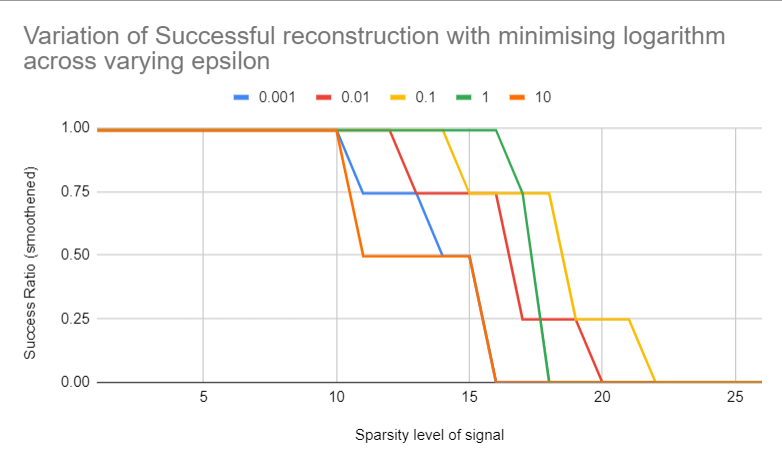
\includegraphics[width=10cm]{log_epsilon.png}
    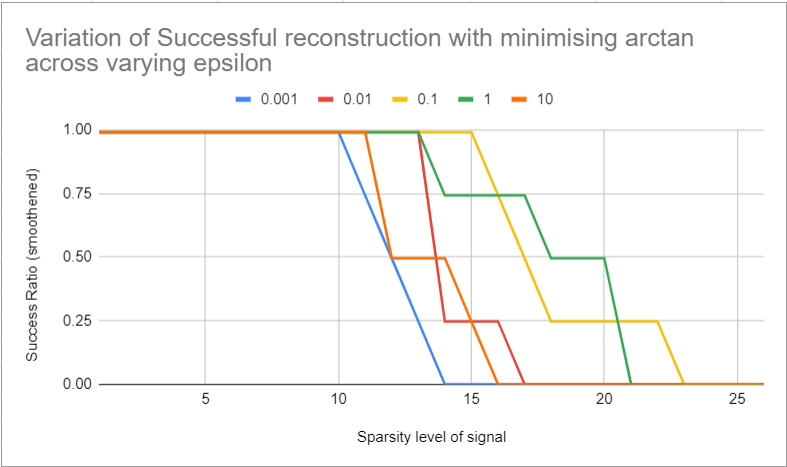
\includegraphics[width=10cm]{atan_epsilon.png}
    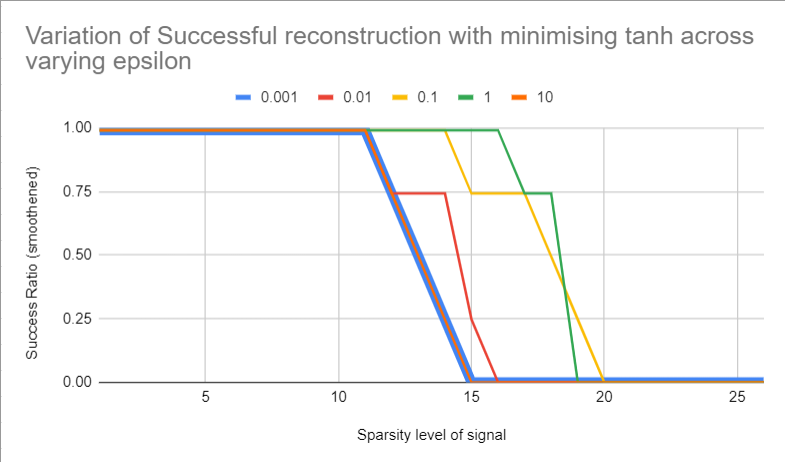
\includegraphics[width=10cm]{tanh_epsilon.png}
    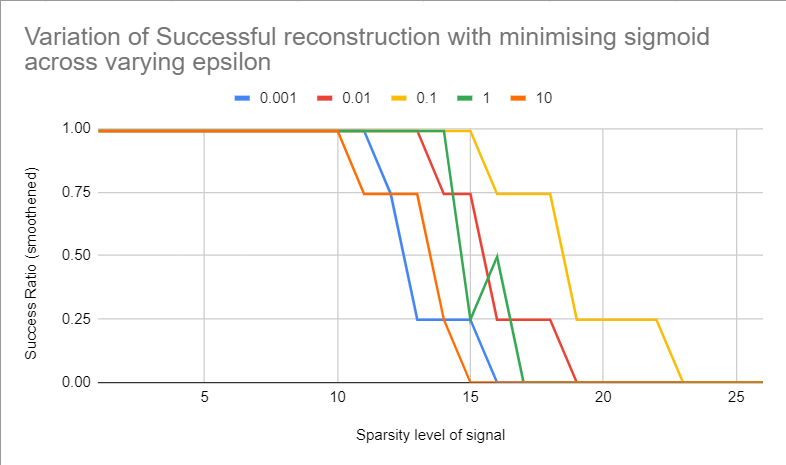
\includegraphics[width=10cm]{sigmoid_epsilon.png}
\end{center}










\subsection{Effect of Number of Reweighting Iterations}
It's obvious that the number of reweighting iterations will improve accuracy. However, our numerical experiments reveal that if convergence occurs, then it usually does so within 2-3 iterations itself, in most cases.

\begin{center}
    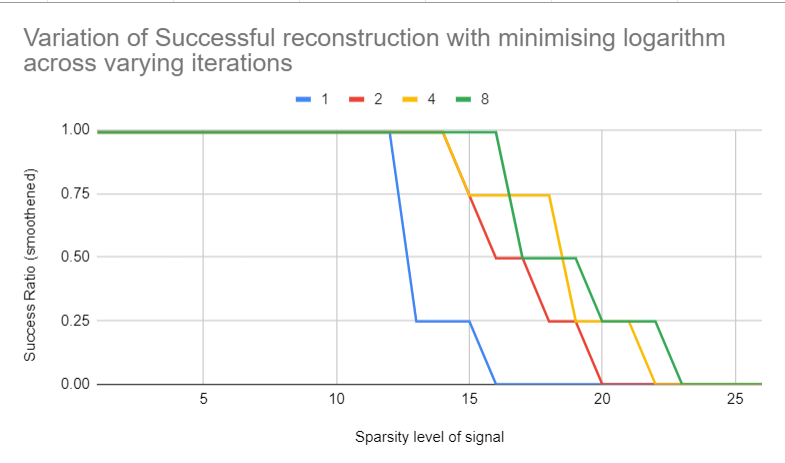
\includegraphics[width=10cm]{log_iterations.png}
    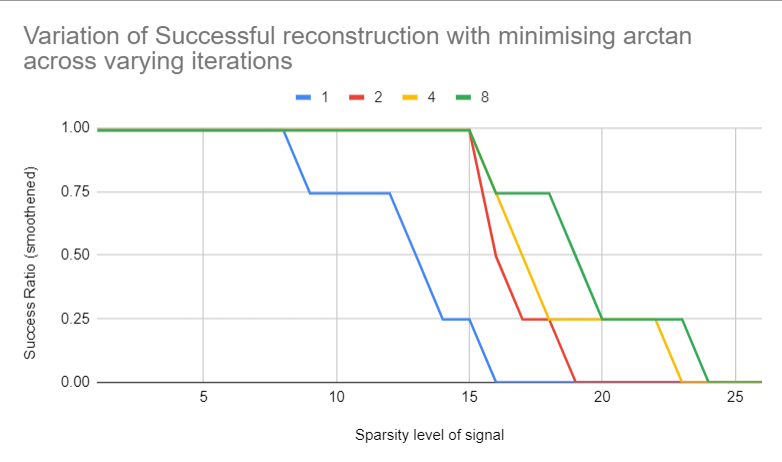
\includegraphics[width=10cm]{atan_iterations.png}
    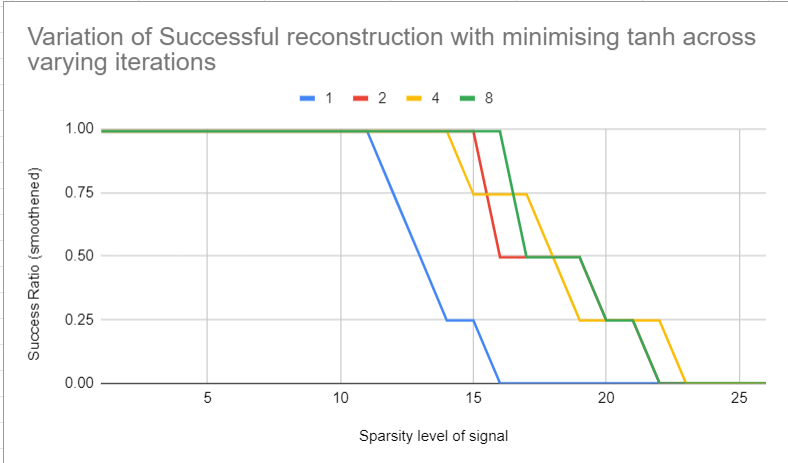
\includegraphics[width=10cm]{tanh_iterations.png}
    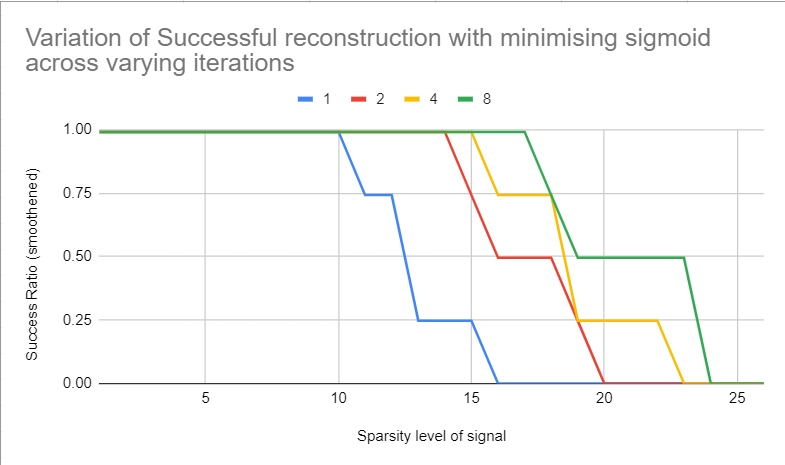
\includegraphics[width=10cm]{sigmoid_iterations.png}
\end{center}


\subsection{Comparison of Times Taken}
As discussed above, a change in the value of $\epsilon$ affects performance a lot. Somewhat surprisingly, it turns out that the value of $\varepsilon$ for which the best recovery probability (the probability of recovery is defined as the proportion of vectors recovered successfully when the same instance of the algorithm, with the same hyperparameters is run multiple times) is obtained, is also the most economical in terms of time taken for execution.

\begin{center}
    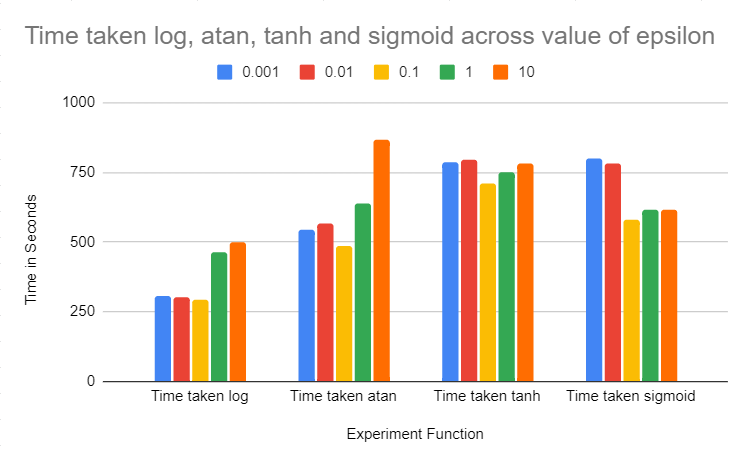
\includegraphics[width=10cm]{time_epsilon.png}
    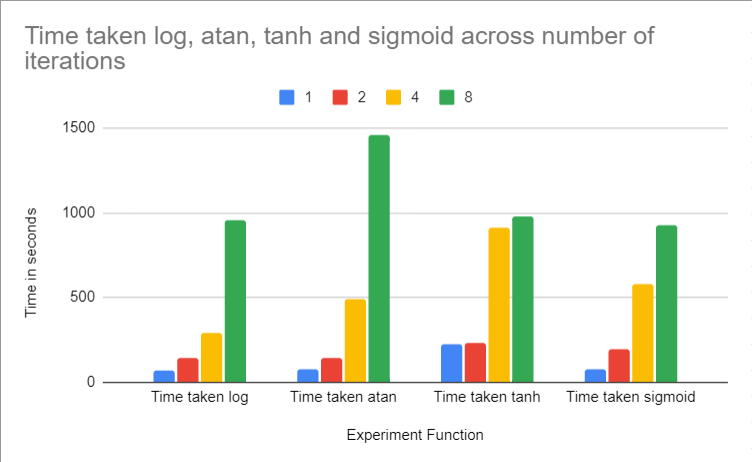
\includegraphics[width=10cm]{time_iterations.png}
\end{center}


\section{Robustness of the Algorithm vis-a-vis Noise}
We observe that more or less same results are obtained even when we consider noisy input, ie:- our relation is now $\boldsymbol{y = \Phi x + \eta}$, where $\boldsymbol{\eta}$ is random Gaussian white noise. While carrying out our numerical experiments though, we observe that we have to relax our threshold for successful recovery somewhat to obtain similar results (we took $\delta = 10^{-3}$ for our noiseless case. For the noisy case we had to relax it to $\delta = 10^{-2}$).

\subsection{Different Cost Functions}

\begin{center}
    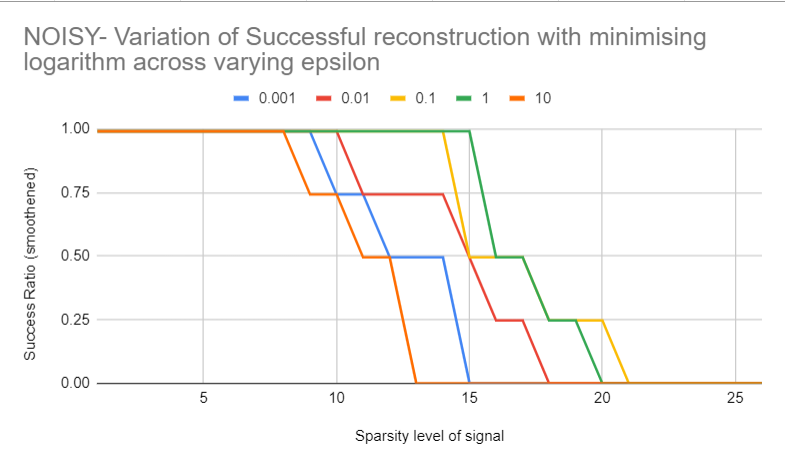
\includegraphics[width=10cm]{log_epsilon_noisy.png}
    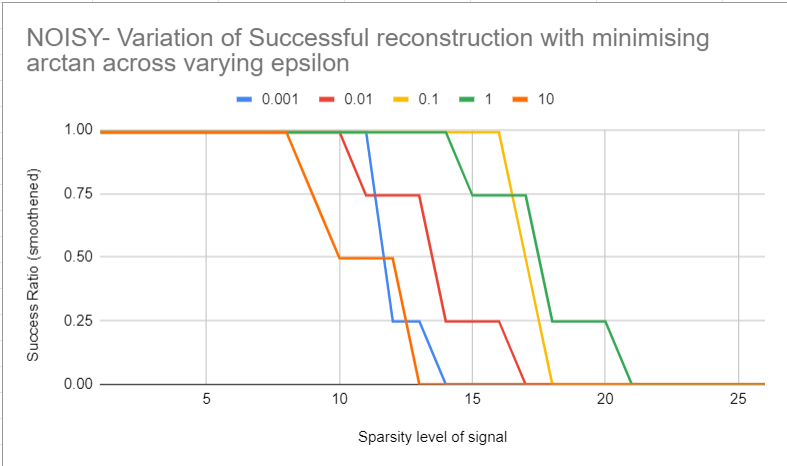
\includegraphics[width=10cm]{atan_epsilon_noisy.png}
    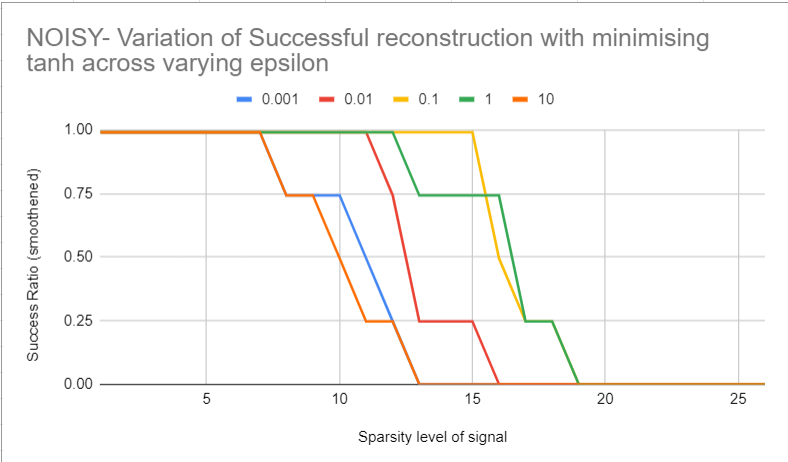
\includegraphics[width=10cm]{tanh_epsilon_noisy.png}
    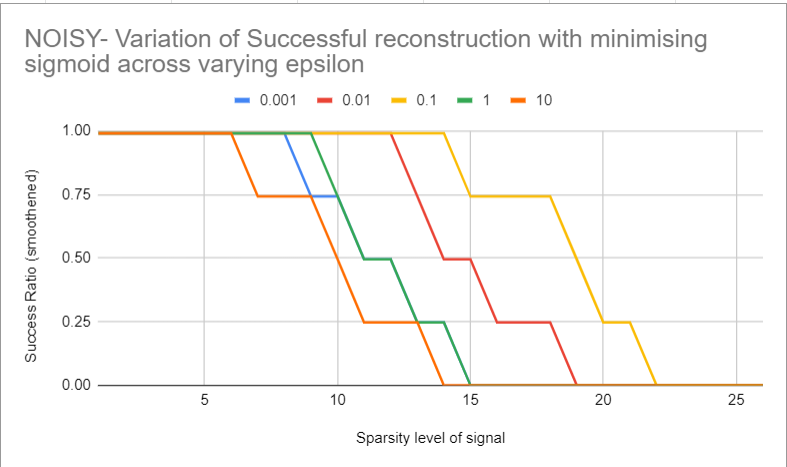
\includegraphics[width=10cm]{sigmoid_epsilon_noisy.png}
\end{center}

\subsection{Effect of Number of Iterations}

\begin{center}
    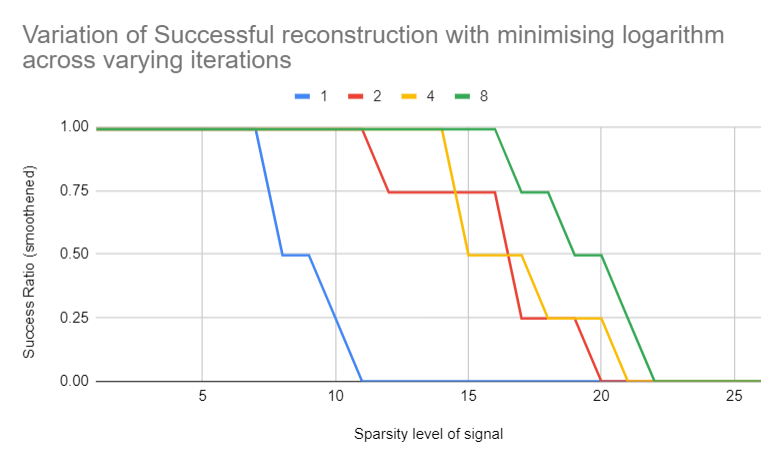
\includegraphics[width=10cm]{log_iterations_noisy.png}
    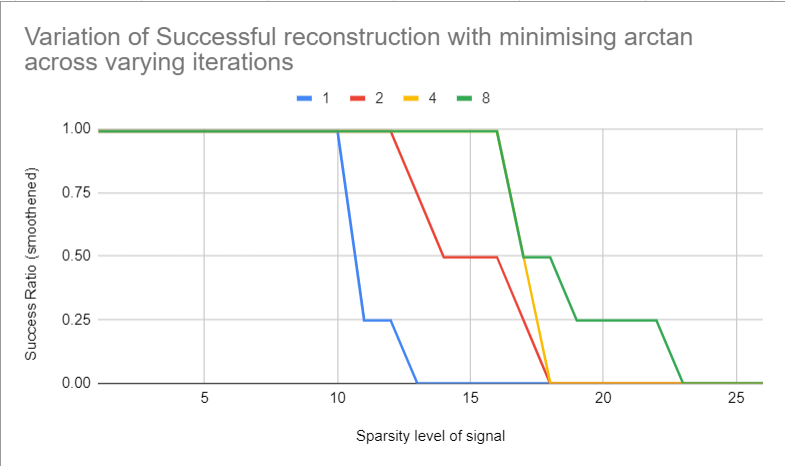
\includegraphics[width=10cm]{atan_iterations_noisy.png}
    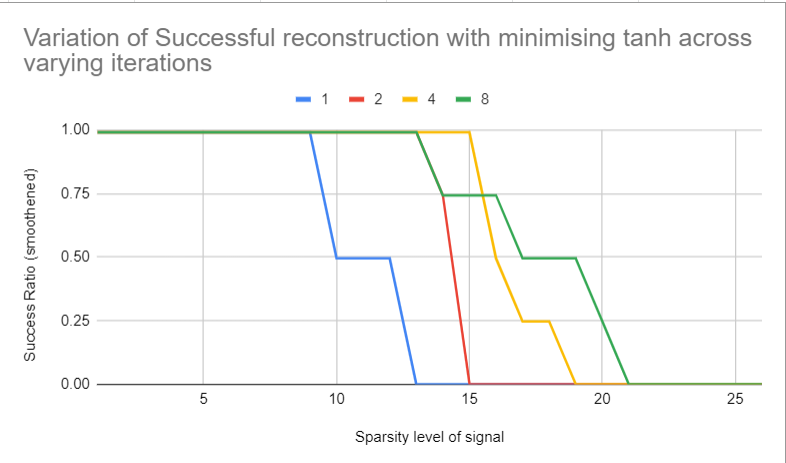
\includegraphics[width=10cm]{tanh_iterations_noisy.png}
    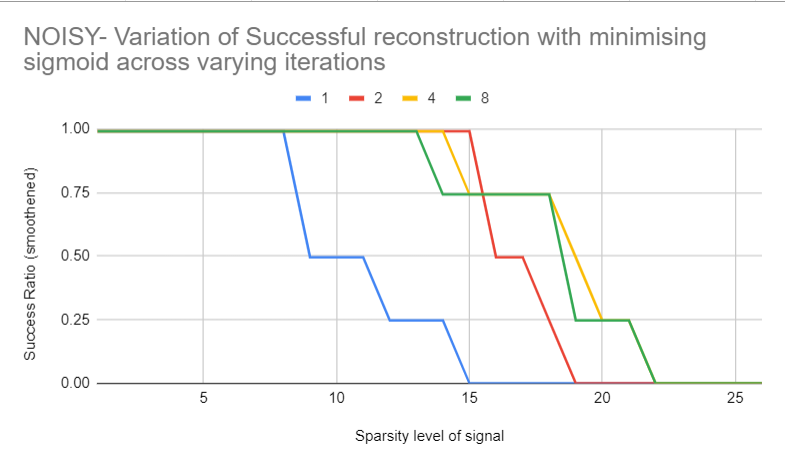
\includegraphics[width=10cm]{sigmoid_iterations_noisy.png}
\end{center}

\subsection{Comparison of Times Taken in Noisy Case}

\begin{center}
    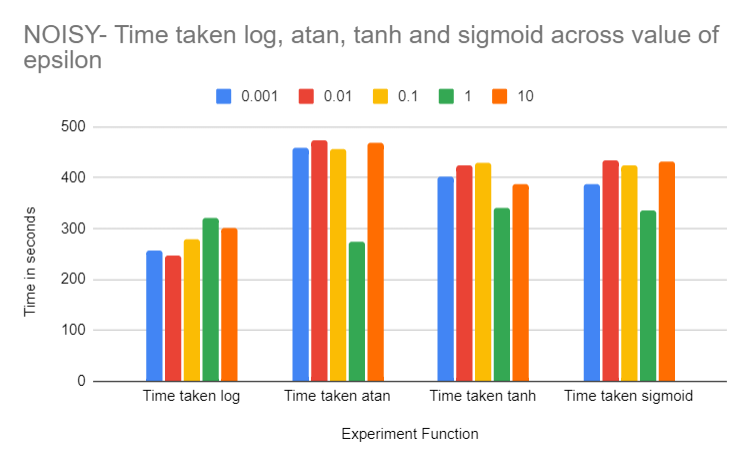
\includegraphics[width=10cm]{time_epsilon_noisy.png}
    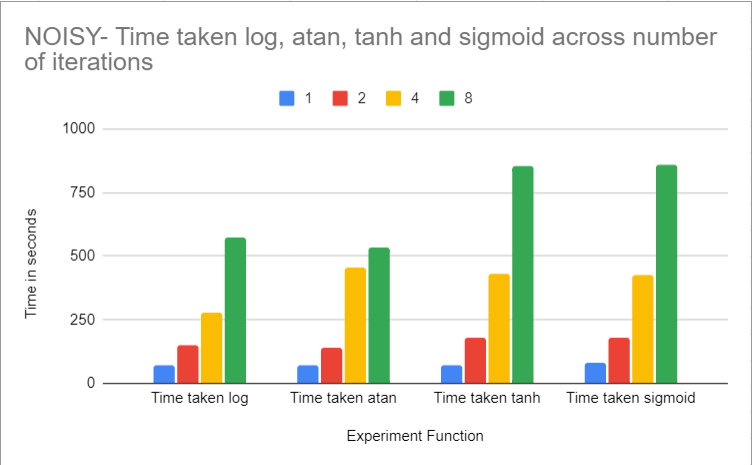
\includegraphics[width=10cm]{time_iterations_noisy.png}
\end{center}

\section{Weeding out Errors: How this algorithm helps in error correcting Codes}
If $m > n$ in $\Phi$, then we enter a field called error correcting codes, in which the sensing matrix is deliberately imbued with some redundancy so as to capture error. Here, instead of minimizing $\boldsymbol{\lVert Wx\rVert_1}$, we minimize $\boldsymbol{\lVert W(y - \Phi x)\rVert_1}$, because here $\boldsymbol{x}$ isn't the sparse quantity, $\boldsymbol{e := y -\Phi x}$ is.\\
The results are more or less in line with the results obtained above.

\begin{center}
    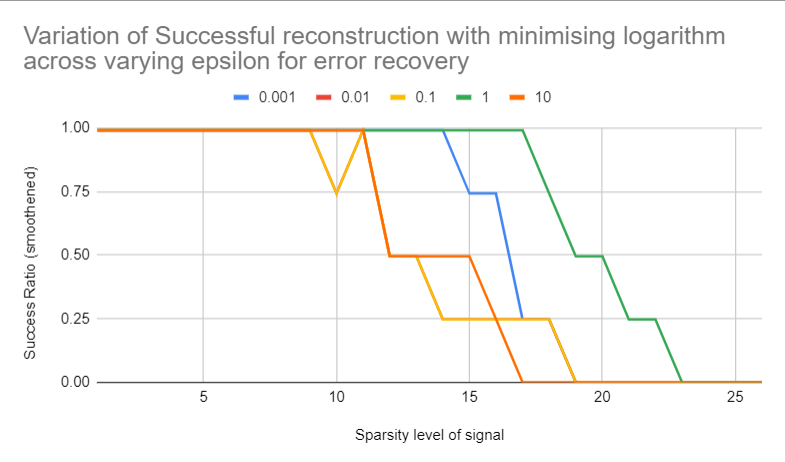
\includegraphics[width=10cm]{Error_Recovery.png}
\end{center}

% \section{Testing Our Algorithm out on Natural Images}










\section{Calculating the exact value of the point sparse recovery breaks down}
As one may observe from the graphs above, the probability of successful recovery \emph{behaves like a phase transition, ie:- after being fairly constant at 1, it suddenly takes a sharp plunge and plummets to 0 within a short interval, displaying interesting transient phenomena in the midst.} Indeed, as we identified, \textbf{the midpoint of the ``transient" region can be taken to be the point of theoretical guarantees, which say that we need $m$ to be atleast $Ck\log (\frac{n}{k})$ for recovery to happen}. This data gives us a numerical way of calculating the constant $C$, as given below.

\begin{center}
    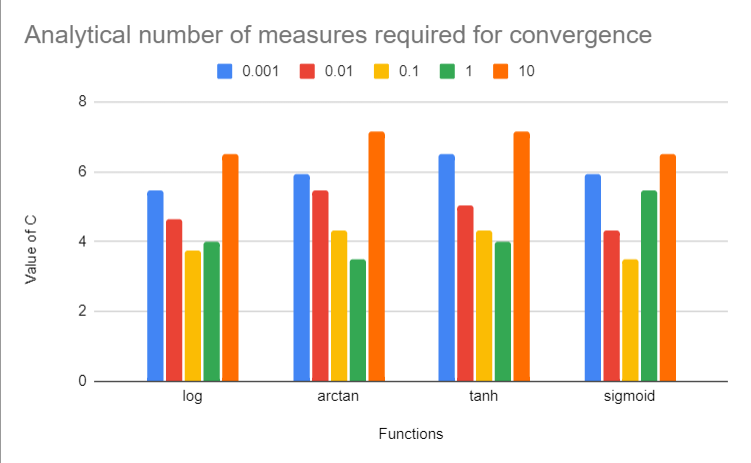
\includegraphics[width=10cm]{constant.png}
\end{center}


\section{Conclusion}

In conclusion, we observe that both concave and convex functions perform similarly in terms of the ability to converge. There is rapid increase in the convergence rate in the second iteration of the weighted L1 norm process itself and further iterations offer only marginal improvement. There seems to a sweet-spot for the hyperparameter where the recovery rate is maximum. Also, this value might differ for the cases with and without noise, as we have already seen above. In conclusion, an iterative approach using several different tools allowed us to better get an intuition of the behaviour of the algorithms.


Thank you for reading.

\end{document}